\documentclass{article}

% Language setting
\usepackage[english]{babel}

% Set page size and margins
\usepackage[letterpaper,top=2cm,bottom=2cm,left=3cm,right=3cm,marginparwidth=1.75cm]{geometry}

% Useful packages
\usepackage[utf8]{inputenc}
\usepackage{latexsym}
\usepackage{amsfonts}
\usepackage{amssymb}
\usepackage{amsthm}
\usepackage{amsmath}
\usepackage{tcolorbox}
\tcbuselibrary{minted}
\usepackage{minted}
\usepackage{mathtools}
\usepackage{float}
\usepackage{natbib}
\usepackage{fourier}
\bibpunct{[}{]}{,}{n}{}{,~}
\usepackage{graphicx}
\usepackage{algorithm}
\usepackage{algpseudocode}

\title{Final exam: Software for Data Science (Julia)}
\author{On the 4$^{th}$ of December 2025 at 2PM}
\date{}

\begin{document}
\maketitle

Find below \textbf{general information} about this final exam:
\begin{itemize}
    \item Duration of \textbf{1 h 30};
    \item One A4 sheet with \textbf{handwritten} notes authorized;
    \item No electronic devices authorized;
    \item There is a total of 5 pages in this exam.
\end{itemize}

\section*{Exercise 1 - Multiple choice}

For each of these \textbf{10 questions}, pick \textbf{one} answer. Multiple answers will be considered to be invalid.

\paragraph{1.} How do you define a function in Julia using assignment syntax?
\begin{itemize}
    \item[A)] \texttt{function add(a, b) return a + b end}
    \item[B)] \texttt{add(a, b) = a + b}
    \item[C)] \texttt{def add(a, b): return a + b}
    \item[D)] \texttt{function add(a, b) = a + b}
\end{itemize}

\medskip
\noindent
\paragraph{2.} What is the purpose of the \texttt{!} at the end of a function name in Julia?
\begin{itemize}
    \item[A)] Indicating the function is asynchronous
    \item[B)] Indicating the function mutates its input arguments
    \item[C)] Indicating the function returns a Boolean
    \item[D)] Indicating the function is deprecated
\end{itemize}

\medskip
\noindent
\paragraph{3.} What is a closure in Julia?
\begin{itemize}
    \item[A)] A function that returns nothing
    \item[B)] A function that captures variables from its surrounding lexical scope
    \item[C)] A function that modifies input arguments
    \item[D)] A function that runs asynchronously
\end{itemize}

\medskip
\noindent
\paragraph{4.} What does the \texttt{throw()} function do in Julia?
\begin{itemize}
    \item[A)] Catches errors
    \item[B)] Creates new variables
    \item[C)] Explicitly raises an error
    \item[D)] Returns a default value
\end{itemize}

\medskip
\noindent
\paragraph{5.} Which data type does Julia infer for the variable \texttt{x} defined as \texttt{x = 3.14}?
\begin{itemize}
    \item[A)] \texttt{Int64}
    \item[B)] \texttt{Float64}
    \item[C)] \texttt{String}
    \item[D)] \texttt{Any}
\end{itemize}

\medskip
\noindent
\paragraph{6.} What is the correct way to broadcast a function \texttt{square} on each element of an array \texttt{vec}?
\begin{itemize}
    \item[A)] \texttt{square(vec)}
    \item[B)] \texttt{square.*(vec)}
    \item[C)] \texttt{square::vec}
    \item[D)] \texttt{square.(vec)}
\end{itemize}

\medskip
\noindent
\paragraph{7.} What does \texttt{Float64 <: Real} mean ?
\begin{itemize}
    \item[A)] \texttt{Real} values should be promoted to \texttt{Float64}
    \item[B)] \texttt{Float64} is a subtype of \texttt{Real}
    \item[C)] \texttt{Real} values are greater than \texttt{Float64} values
    \item[D)] Values in $\mathbb{R}$ are represented exactly in Julia
\end{itemize}

\medskip
\noindent
\paragraph{8.} What does it mean to compile a program ?
\begin{itemize}
    \item[A)] To put together functions in a same file
    \item[B)] To execute the prorgam on a CPU
    \item[C)] To improve performance of a program
    \item[D)] To generate the CPU instructions from a program
\end{itemize}

\medskip
\noindent
\paragraph{9.} What is the \texttt{export} keyword used for in a \texttt{Module} in Julia ?
\begin{itemize}
    \item[A)] To compile the module
    \item[B)] To indicate functions from the module that are public
    \item[C)] To indicate functions from the module that are private
    \item[D)] To have access to functions from other modules
\end{itemize}

\medskip
\noindent
10. What does \texttt{isconcretetype(Any)} return ?
\begin{itemize}
    \item[A)] \texttt{Number}
    \item[B)] \texttt{String}
    \item[C)] \texttt{false}
    \item[D)] \texttt{true}
\end{itemize}

\section*{Exercise 2 - Dijkstra’s Algorithm}

In this exercice, we consider a directed graph, i.e. a graph in which the vertices are linked through oriented edges. The aim is to implement \textbf{Dijkstra’s Algorithm} in order to determine the shortest path distances from the source vertex, with identifier 1, to all other vertices in the graph. Let us use the \texttt{Graphs.jl} package to represent the graph. 

\begin{tcblisting}{listing engine=minted, minted language=julia, colback=gray!10, colframe=black, listing only}
using Graphs
\end{tcblisting}

\paragraph{Question 1} \textit{In the rest of this exercise we will consider to be working in a script, not in the REPL. Write the instructions to activate local environment. Add the \texttt{Graphs.jl} package.}

\medskip
\noindent
Find below an extract of the documentation for generating a directed graph using \texttt{Graphs.jl}.

\begin{tcblisting}{listing engine=minted, minted language=julia, colback=gray!10, colframe=black, listing only}
help?> SimpleDiGraph
search: SimpleDiGraph SimpleGraph CompleteDiGraph CompleteGraph CycleDiGraph WheelDiGraph

  SimpleDiGraph{T}

  A type representing a directed graph.
  ________________________________________________________________________________

  SimpleDiGraph{T}(n=0)

  Construct a SimpleDiGraph{T} with n vertices and 0 edges. If not specified, the element
  type T is the type of n.

  Examples
  ========

  julia> using Graphs
  
  julia> SimpleDiGraph(UInt8(10))
  {10, 0} directed simple UInt8 graph
\end{tcblisting}

\medskip
\noindent
The oriented edges linking together the vertices of the graph \texttt{g} are defined using \texttt{add\_edge!}. Find the documentation below.

\begin{tcblisting}{listing engine=minted, minted language=julia, colback=gray!10, colframe=black, listing only}
help?> add_edge!
search: add_edge! rem_edge! add_vertex! has_edge add_vertices! add_edge_checked!

  add_edge!(g, e)

  Add an edge e to graph g. Return true if edge was added successfully, otherwise return false.

  Examples
  ========

  julia> using Graphs
  
  julia> g = SimpleGraph(2);
  
  julia> add_edge!(g, 1, 2)
  true
\end{tcblisting}

\medskip
\noindent
In the rest of this exercise, the \textbf{graph} we will be working on is the one with \textbf{five vertices} presented below. Pay attention to the orientation of the edges. Note that the vertices accessible from a given vertex are reffered to as its neighbours.

\medskip
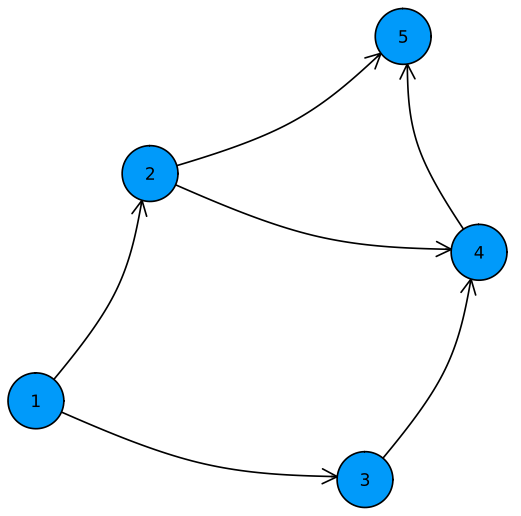
\includegraphics[scale=0.4]{graph.png}

\medskip
\paragraph{Question 2} \textit{Write the instructions in Julia to define the graph provided in the figure based on the functions defined before.}

\medskip
\noindent
Let us present \textbf{Dijkstra’s algorithm}. It consists of computing the minimal distance between the source vertex 1 and each vertex in the graph while keeping track of which vertex we came from to minimize that distance. Alternatively, the vertices of the graph will be stored in the \texttt{to\_visit} and \texttt{visited} array. Since extra information can not directly be attached to the vertices in the graph, we will store additional informal in a \texttt{properties} dictionnary. The information that will be associated to each vertex index is:

\begin{itemize}
    \item \texttt{min\_d} which represents the minimal distance to the source vertex; 
    \item \texttt{id\_pre} which represents the predecessor vertex through which the shortest path goes.
\end{itemize}

\noindent
The \textbf{distance} to go from one vertex to another through \textbf{one edge is 1}. Read carefully the algorithm below to understand how these arrays and this dictionnary are used.

\medskip
\noindent
\begin{tcolorbox}[colframe=black,colback=white,title=Dijkstra’s Algorithm]
\begin{algorithmic}[1]
  \item[(Step 1)] Add the starting vertex 1 to the \texttt{to\_visit} array. Store the associated information, i.e. the distance \texttt{0} and predecessor \texttt{-1}, in the \texttt{properties} dictionary.
  
  \item[(Step 2)] While \texttt{to\_visit} is not empty, do:
  \begin{algorithmic}[1]
    \item[(Step 2.1)] Take the first vertex \texttt{v\_c} in \texttt{to\_visit}.

    \item[(Step 2.2)] Remove \texttt{v\_c} from the \texttt{to\_visit} array.

    \item[(Step 2.3)] Add \texttt{v\_c} to the \texttt{visited} array.
    
    \item[(Step 2.4)] For each neighbor \texttt{v\_n} of \texttt{v\_c} which is not in the \texttt{visited} array, do:
    \begin{algorithmic}[1]
      \item[(Step 2.4.1)] Add \texttt{v\_n} to the \texttt{to\_visit} array, if not done yet.

      \item[(Step 2.4.2)] Compute the total distance \texttt{$\tilde{\delta}$} from the source to \texttt{v\_n} passing through \texttt{v\_c}. Let \texttt{$\delta_{v\_c}$} be the optimal distance from the source to \texttt{v\_c}. Then \texttt{$\tilde{\delta}$ = $\delta_{v\_c}$ +1}.

      \item[(Step 2.4.3)] Initialize an entry, with \texttt{$\tilde{\delta}$} and \texttt{v\_c}, for \texttt{v\_n} in the \texttt{properties} dictionary, if not done yet.
      
      \item[(Step 2.4.4)] If \texttt{$\tilde{\delta}$ < $\delta_{v\_n}$}, then \texttt{v\_c} is a better predecessor for \texttt{v\_n}. Update the information associated to \texttt{v\_n} in the the \texttt{properties} dictionary.
    \end{algorithmic}
  \end{algorithmic}
\end{algorithmic}
\end{tcolorbox}

\medskip
\noindent
Once this algorithm finishes, \texttt{visited} contains all the vertices reachable from the source, and for every vertex in \texttt{visited}, the distance is optimal. To implement the algorithm, let us start by setting up some utilitaries.

\newpage
\noindent
Find below \textbf{the notes of a student} that applied this algorithm to the graph with five vertices presented before.

\medskip
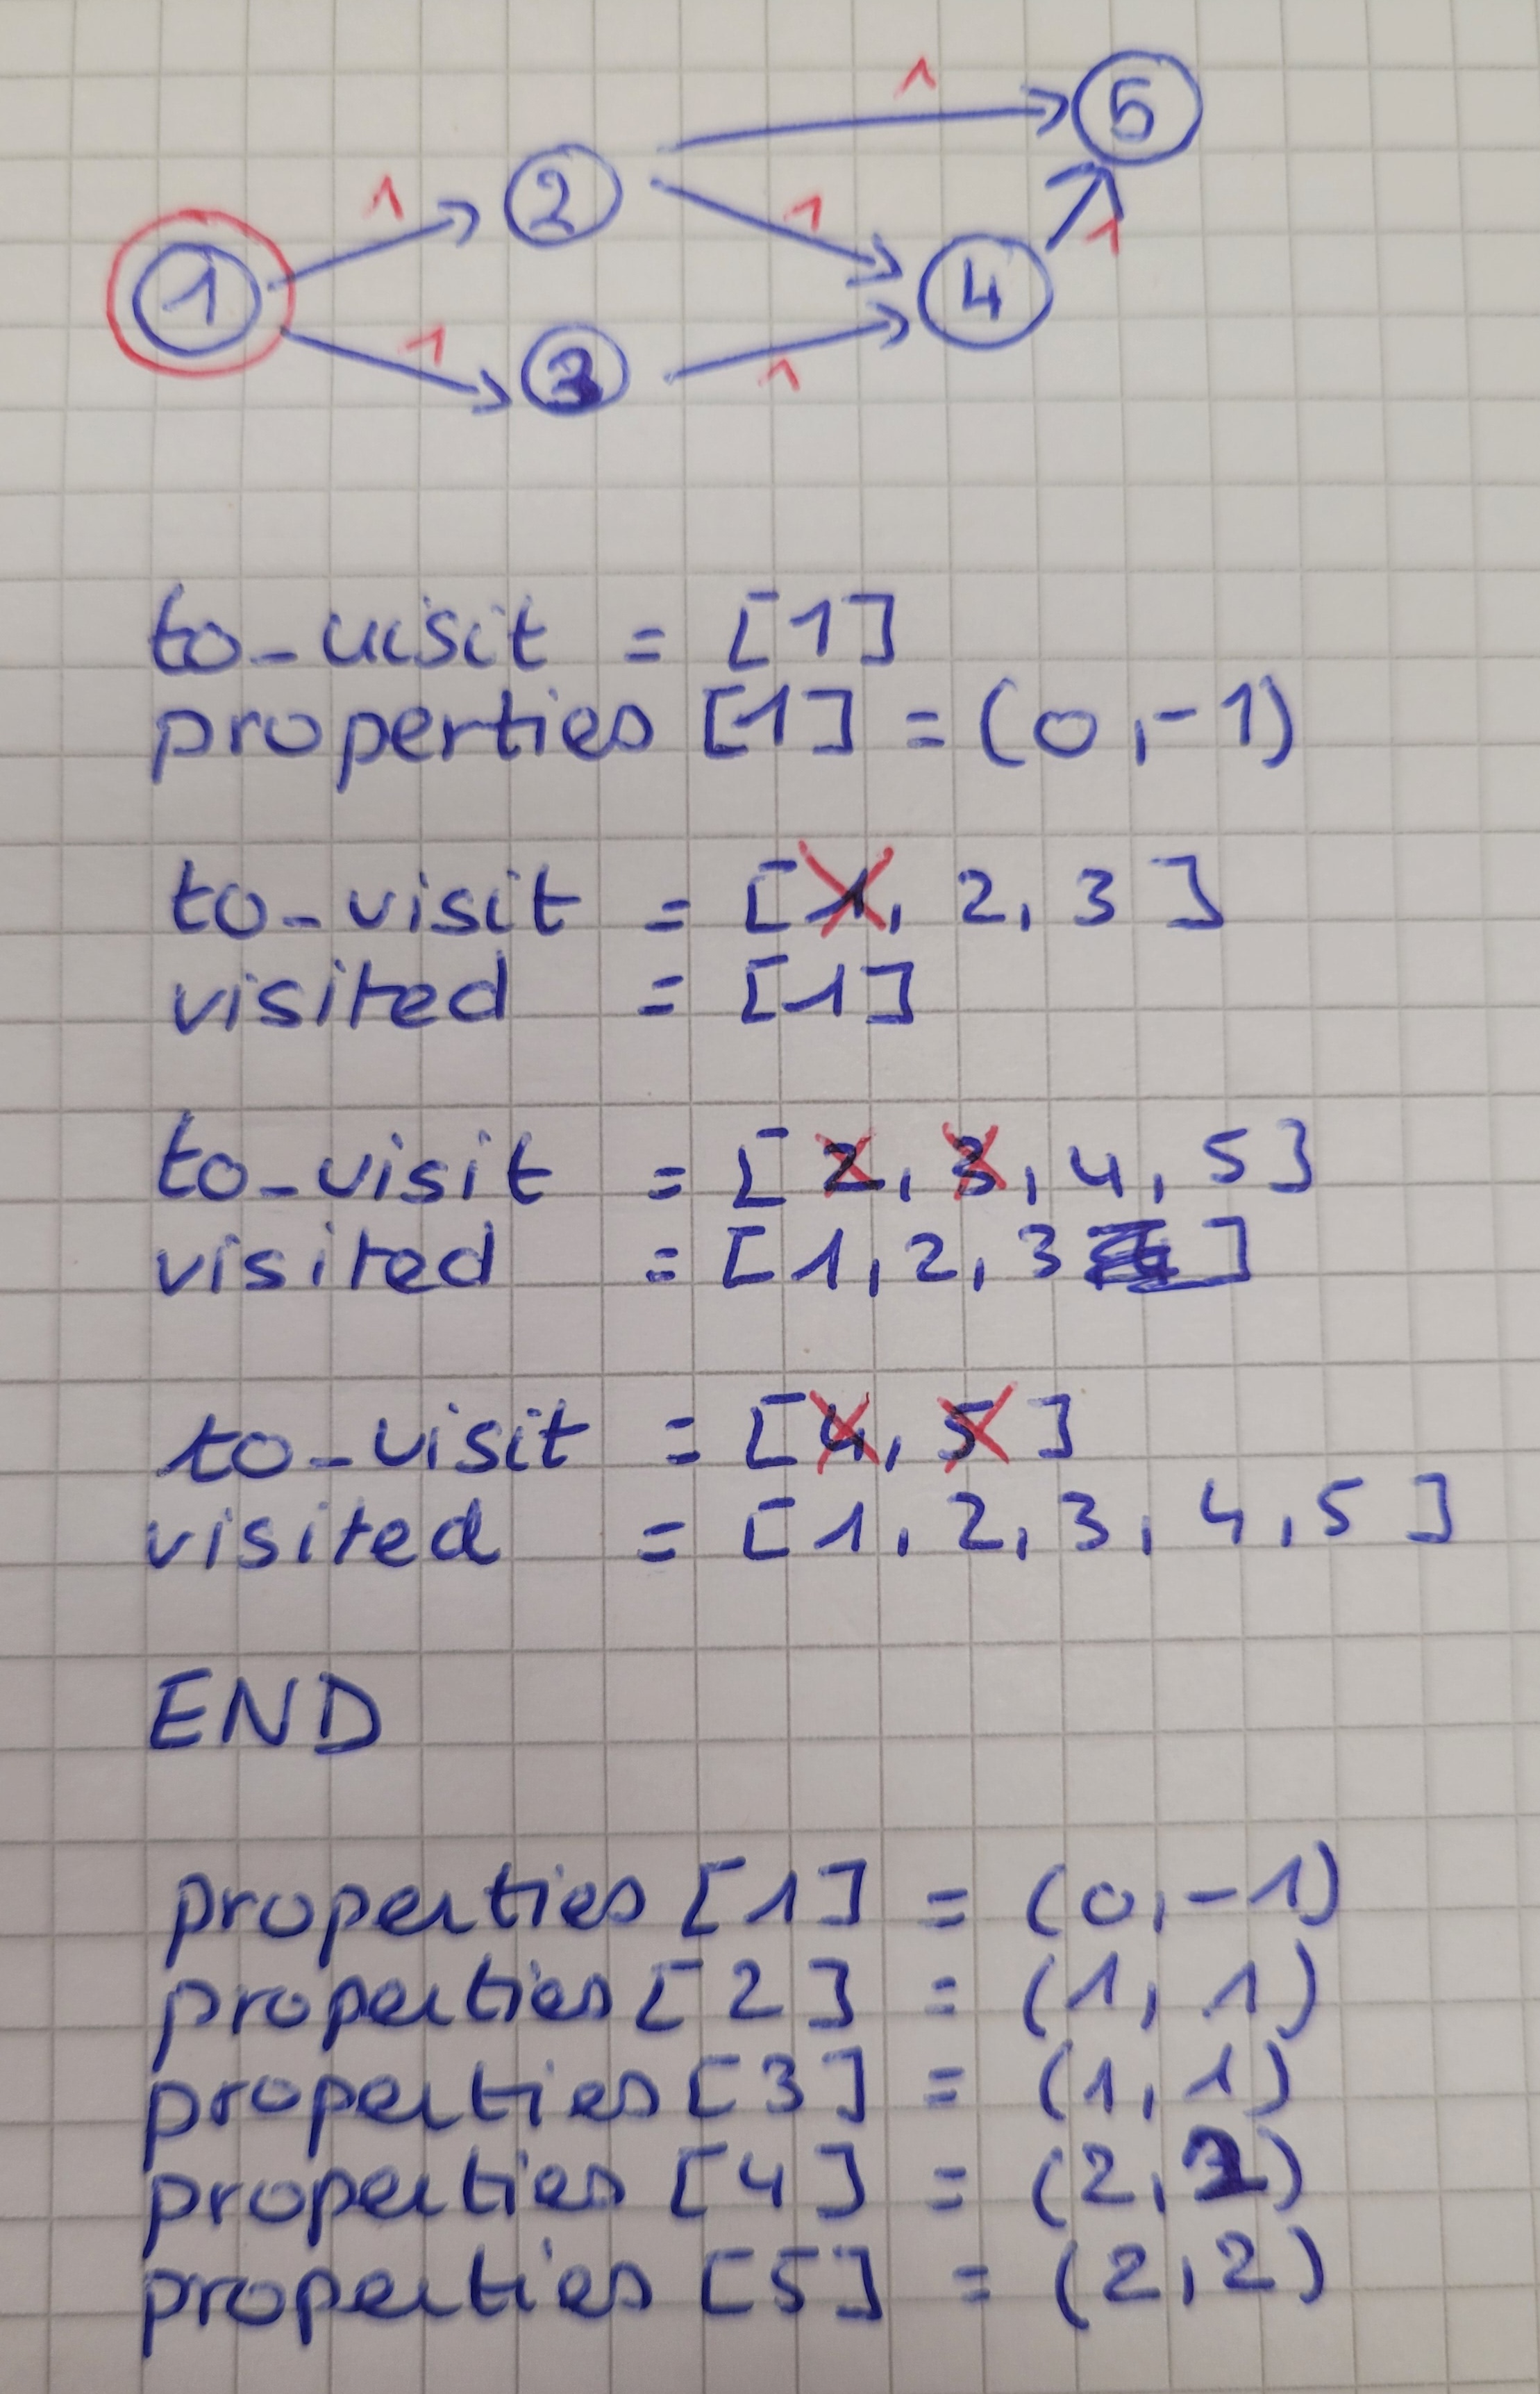
\includegraphics[scale=0.075]{student.jpg}

\noindent
\paragraph{Question 3} \textit{Identify the steps from the algorithm in the notes of the student. Comment providing step labels and associate variable names to the values in the notes.}

\medskip
\noindent
Let us get back to \textbf{Julia}.

\paragraph{Question 4} \textit{Create your own type to hold the distance and predecessor information associated to each vertex. This structure will later be stored in the \texttt{properties} dictionary. Recall that the attributes of this structure are updated by the Dijkstra algorithm.}

\paragraph{Question 5} \textit{Create the \texttt{properties} dictionary. Initialize it for the source vertex 1 as in step 1 in the above algorithm. Use the structure created in the previous question to store the data.}

\paragraph{Question 6} \textit{Which control loop and condition to use for (Step 2) ? Write down the structure of the loop. The code inside the loop is not asked for in this question.}

\medskip
\noindent
The first element of the \texttt{to\_visit} has to be removed in step 2.2. Note that \texttt{deleteat!(to\_visit, pos)} deletes the element from the \texttt{to\_visit} array which is at the position \texttt{pos}. 

\paragraph{Question 7} \textit{What is the value of the first index of an array in Julia ?}

\medskip
\noindent
Step 2.4 in the algorithm requires to access the neighbour vertices of \texttt{v\_c}. To access the indentifiers of the neighbors use \texttt{neighbors(g, v\_c)}.

\paragraph{Question 8} \textit{Write in Julia the loop of (Step 2.4).}

\paragraph{Question 9} \textit{In step 2.4.1, the current neighbor should be added to \texttt{to\_visit}, if not yet done. How to add an element to the end of an array in Julia ?}

\medskip
\noindent
In order to check whether the identifier of a vertex is present in the \texttt{properties} dictionary for step 2.4.3, use the command \texttt{keys(properties)} which returns all the keys within the dictionnary \texttt{properties}.

\paragraph{Question 10} \textit{Write in Julia the condition to check wether a given key is NOT yet in the dictionnary.}

\paragraph{Question 11} \textit{Implement the whole algorithm.}

\end{document}